% -----------------------------------------------------------------------------
% Resultados
% -----------------------------------------------------------------------------

\chapter{Result Analysis and Discussion - BNE}
\label{chap:Resultados-BNE}

%Cada capítulo deve conter uma pequena introdução (tipicamente, um ou dois parágrafos), em seção não numerada, que deve deixar claro o objetivo e o que será discutido no capítulo, bem como a organização do capítulo.

%\section{Título da seção}
%\label{sec:titSecResult}

%Inserir seu texto aqui...

    Nesta parte da tese, utilizaremos 2500 grãos. O diâmetro médio do grão é $d = 1\pm 2.5\%$, distribuídos uniformemente. O diâmetro do intruso é de $D = 5$ vezes o diâmetro médio dos grãos. A densidade de todos os grãos é a mesma, e vale $\rho = 1/\pi$, e portanto a massa média dos grãos é de $m = 0,25$, exceto quando estiver ressaltado nas figuras. A constante de mola na direção normal é de $k_{n} = 1000$ e a tangencial é de $k_{t} = 750$. A atuação do amortecedor é no regime crítico ($\gamma = 2\sqrt{m k}$), e vale aproximadamente $\gamma = \sqrt{10}$. O atrito dos grãos valem $\mu = 0,5$, tanto entre grãos, quanto entre paredes, quando houver. O passo de tempo ($dt=pT$) vale aproximadamente $dt = \frac{1}{2000\sqrt{10}}$, utilizando a fração de $p=0,01$ do período de oscilação do modelo de contato massa mola $T = \sqrt{\frac{m}{k}}$. A largura da caixa é de $L = 37.5$ diâmetros de grão.

    Inicialmente, estudamos o sistema com paredes no fundo e nas laterais, formando uma caixa. Observamos nestas simulações correntes de convecção próximos às paredes.

\begin{figure}
    \centering
    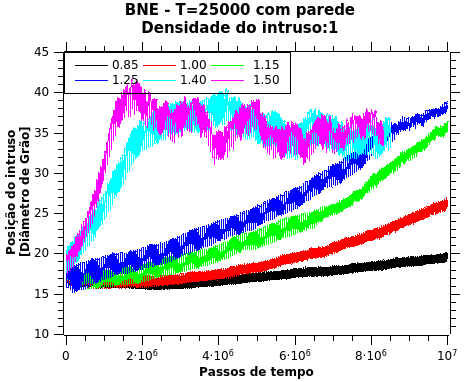
\includegraphics[width=0.45\textwidth]{04-figuras/BNE25000D1.png}
    \caption{Média de 10 amostras da subida do intruso em função do adimensional de aceleração. O período de agitação é de 25000 passos de tempo em uma forma senoidal. Este sistema possui atrito nas paredes e densidade do intruso igual a dos grãos.}
    \label{fig:BNE25000_Parede}
\end{figure}

\begin{figure}
    \centering
    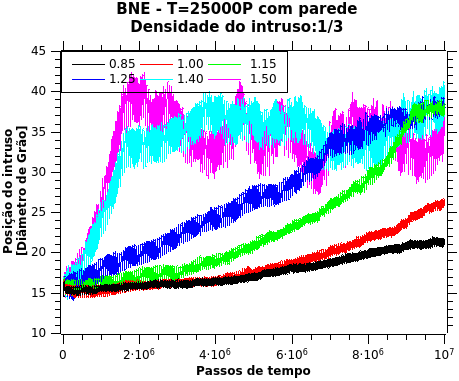
\includegraphics[width=0.45\textwidth]{04-figuras/BNE25000D1-3.png}
    \caption{Média de $5$ amostras da subida do intruso em função do adimensional de aceleração. O período de agitação é de $25000$ passos de tempo em uma forma senoidal. Este sistema possui atrito nas paredes e densidade do intruso é $\frac{1}{3}$ da densidade dos grãos.}
    \label{fig:BNE25000_Parede_Densidade1-3}
\end{figure}

\begin{figure}
    \centering
    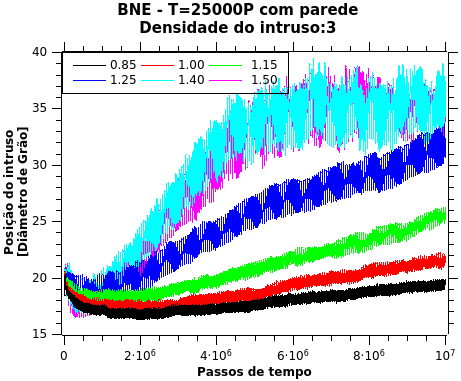
\includegraphics[width=0.45\textwidth]{04-figuras/BNE25000D3.png}
    \caption{Média de $5$ amostras da subida do intruso em função do adimensional de aceleração. O período de agitação é de $25000$ passos de tempo em uma forma senoidal. Este sistema possui atrito nas paredes e densidade do intruso é $3$ vezes a densidade dos grãos.}
    \label{fig:BNE25000_Parede_Densidade3}
\end{figure}

    Percebemos que intrusos mais densos sobem mais lentamente que intrusos menos densos. Os tempos de subida, quando comparados, podem ser ordenados das figuras $\ref{fig:BNE25000_Parede_Densidade1-3} < \ref{fig:BNE25000_Parede} < \ref{fig:BNE25000_Parede_Densidade3}$. Assim como as correntes de convecção são mais intensas, o intruso sobe mais rapidamente e cai mais rapidamente, visto na amplitude de $\Gamma = 1,5$ para as figuras \ref{fig:BNE25000_Parede_Densidade1-3}, \ref{fig:BNE25000_Parede} e \ref{fig:BNE25000_Parede_Densidade3}, respectivamente.

    Quando retirado o atrito entre os grãos e as paredes, temos que o efeito da convecção no sistema diminui, ocasionando em uma subida mais lenta que quando o atrito está presente. A figura \ref{fig:BNE25000_sem_Atrito_Parede} mostra a subida do intruso no sistema em que as paredes não possuem atrito.

\begin{figure}
    \centering
    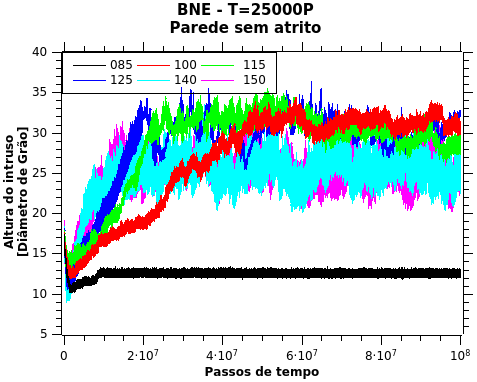
\includegraphics[width=0.45\textwidth]{04-figuras/BNE25000PsemAtrito.png}
    \caption{Média de $3$ amostras da subida do intruso em função do adimensional de aceleração. O período de agitação é de $25000$ passos de tempo em uma forma senoidal. Este sistema não possui atrito nas paredes.}
    \label{fig:BNE25000_sem_Atrito_Parede}
\end{figure}

    Ao comparar os tempos de subida do sistema que possui atrito nas paredes (figura \ref{fig:BNE25000_Parede}) com o sistema que não possui atrito nas paredes (figura \ref{fig:BNE25000_sem_Atrito_Parede}), percebemos que o tempo de subida é maior, além de que o sistema que possui agitação menor que a gravidade não sobe, mostrando que um dos fatores que importam para o \textit{BNE} são as correntes de convecção formadas próximas das paredes.

    Quando retiramos o atrito do sistema, o intruso chega ao fundo do sistema, independente da amplitude de vibração. A figura \ref{fig:BNE25000_sem_Atrito} exibe o comportamento do intruso para o sistema sem atrito.

\begin{figure}
    \centering
    \begin{minipage}{.45\linewidth}
        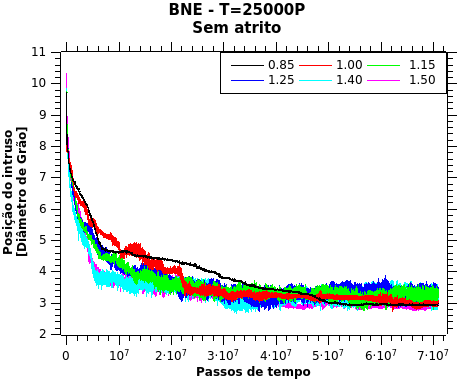
\includegraphics[width=0.9\textwidth]{04-figuras/BNE25000semAtrito.png}
        \subcaption{Diferentes amplitudes}
        \label{fig:BNE25000_sem_Atrito_Sistema}
    \end{minipage}
    \begin{minipage}{.45\linewidth}
        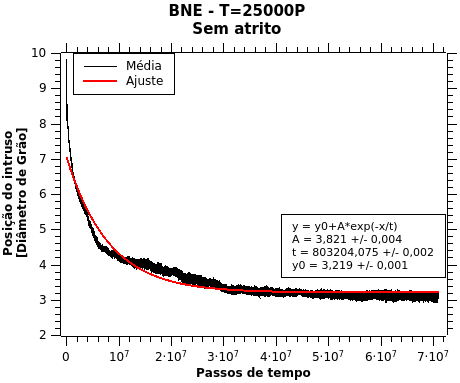
\includegraphics[width=0.9\textwidth]{04-figuras/BNE25000semAtrito_Ajuste.png}
        \subcaption{Ajuste da média}
        \label{fig:BNE25000_sem_Atrito_Ajuste}
    \end{minipage}
    \caption{Amostra da queda do intruso em função do adimensional de aceleração. O período de agitação é de $25000$ passos de tempo em uma forma senoidal. Este sistema não possui atrito. A figura \ref{fig:BNE25000_sem_Atrito_Ajuste} possui a média das curvas apresentadas na figura \ref{fig:BNE25000_sem_Atrito_Sistema} e uma o ajuste de um decaimento exponencial em função do tempo, da posição do intruso até o fundo do sistema.}
    \label{fig:BNE25000_sem_Atrito}
\end{figure}

    Se ao invés de retirarmos o atrito, retirarmos as paredes laterais formando uma condição periódica de contorno de largura $28$ diâmetros de grão, verificaremos que o \textit{BNE} não acontece para o período de vibração de $25000$ passos de tempo, como mostrado na figura \ref{fig:BNE25000_Contorno}.

\begin{figure}
    \centering
    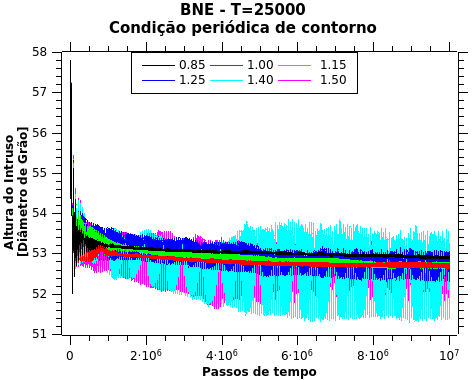
\includegraphics[width=0.45\textwidth]{04-figuras/BNE25000Contorno.png}
    \caption{Média de $5$ amostras da posição do intruso em função do adimensional de aceleração. O período de agitação é de $25000$ passos de tempo em uma forma senoidal. Este sistema não possui paredes, mas condição periódica de contorno.}
    \label{fig:BNE25000_Contorno}
\end{figure}

    Já no caso de períodos maiores, o BNE ocorre. A figura \ref{fig:BNE30000_Contorno} exemplifica o \textit{BNE} ocorrendo com condição periódica de contorno e período de vibração de $30000$ passos de tempo.

\begin{figure}
    \centering
    \begin{minipage}{.45\linewidth}
        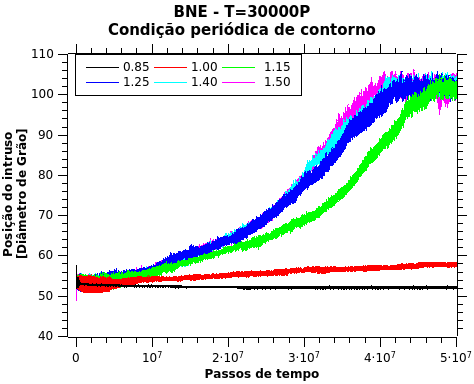
\includegraphics[width=0.9\textwidth]{04-figuras/BNE30000Contorno.png}
        \subcaption{Média das amostras}
        \label{fig:BNE30000_Contorno_Media}
    \end{minipage}
    \begin{minipage}{.45\linewidth}
        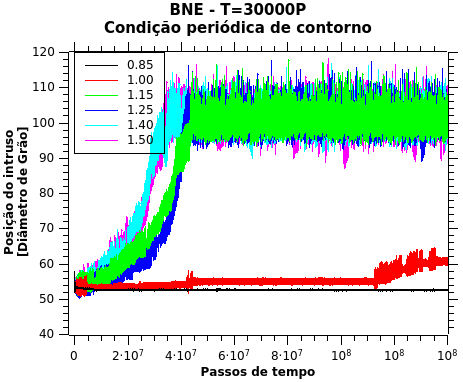
\includegraphics[width=0.9\textwidth]{04-figuras/BNE30000Contorno1.png}
        \subcaption{Amostra mais longa}
        \label{fig:BNE30000_Contorno1}
    \end{minipage}
    \caption{Média de $10$ amostras da subida do intruso em função do adimensional de aceleração. O período de agitação é de $30000$ passos de tempo em uma forma senoidal. Este sistema não possui paredes, mas condição periódica de contorno. A figura \ref{fig:BNE30000_Contorno1} mostra a amostra com maior passos de tempo de simulação.}
    \label{fig:BNE30000_Contorno}
\end{figure}

    Na figura \ref{fig:BNE30000_Contorno1}, percebemos que acelerações menores que a gravidade não fazem o intruso ascender, enquanto acelerações próximas da gravidade tem um movimento de ascensão lento e em saltos. Por não haver paredes, as correntes de convecção não se formam no sistema, o que faz com que o intruso atinja o topo e não desça mais.

%    Com estes resultados, submetemos um artigo para a publicação ... \textbf{Parte necessária para a qualificação}.

    No próximo capítulo, descreveremos os modos de transporte de grãos quando arrastados por um fluido.
